\addtocontents{toc}{\protect\setcounter{tocdepth}{0}}
\addtotoc{Management Summary}
\chapter*{Management Summary}
In this project, we try to incorporate spatial data representations in OpenRefine by the examples of integrating
OpenStreetMap data into OpenRefine and being able to export OpenRefine data to the GeoJSON (.geojson) format.
Two extensions are built for achieving such goals.
\section*{Goals}
\subsection*{The OSM Extractor Extension}
For the OSM Extractor extension, these are the goals:
\begin{enumerate}
    \item Build an OpenRefine extension using OpenRefine\textquotesingle s extension architecture
    \item The extension must be able to utilize the Overpass API and other different OpenStreetMap Java libraries to successfully
    integrate OpenStreetMap data into OpenRefine
    \item The OpenStreetMap elements must be converted to \text{Simple Feature} geometry before being inserted to OpenRefine
    \item The extension\textquotesingle s forms and dialogs must be user-friendly and the process of integrating data must be as efficient
    and as least-effort as possible (for the user)
\end{enumerate}
\subsection*{The GeoJSON Export Extension}
For the GeoJSON Export extension, these are the goals:
\begin{enumerate}
    \item Build an OpenRefine extension using OpenRefine\textquotesingle s extension architecture
    \item The extension must be able to export data of an OpenRefine project into the GeoJSON (.geojson) format. Latitude/Longitude
    can be used for exporting \mintinline{bash}{Points} and WKT strings can be used for exporting any type of \textit{Simple Feature} geometry.
    A combination of both can be used for exporting
    \item The extension\textquotesingle s forms and dialogs must be user-friendly and the process of exporting data must be as efficient
    and as least-effort as possible (for the user)
\end{enumerate}
\pagebreak
\section*{Results}
\subsection*{The OSM Extractor Extension}
The extension has been successfully developed using OpenRefine\textquotesingle s extension architecture and is able to successfully
integrate OpenStreetMap data (as Simple Features) into a new OpenRefine project.
\begin{figure}[H]
        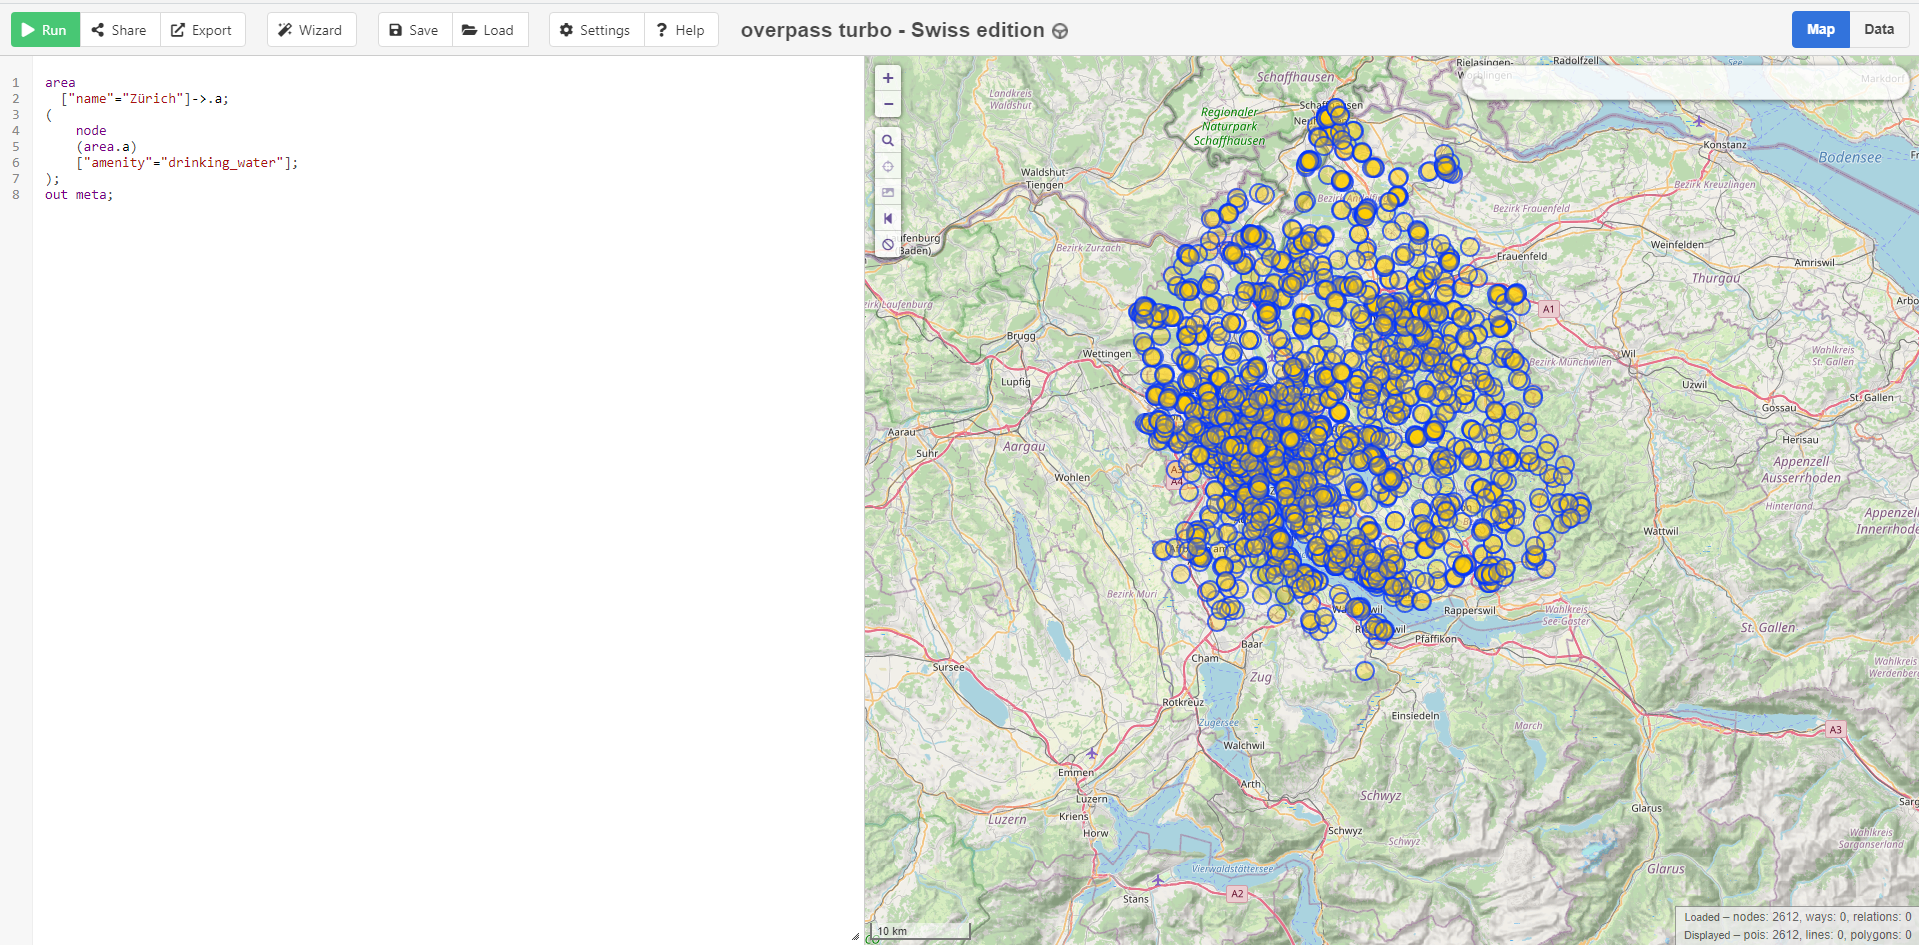
\includegraphics[width=\textwidth]{./Figures/ManagementSummary/osm_extractor_overpass_query}
        \caption{OpenStreetMap data for all the drinking water amenities in Zürich, Switzerland, taken from \href{http://overpass-turbo.osm.ch/}{Overpass Turbo CH}}
\end{figure}
\begin{figure}[H]
    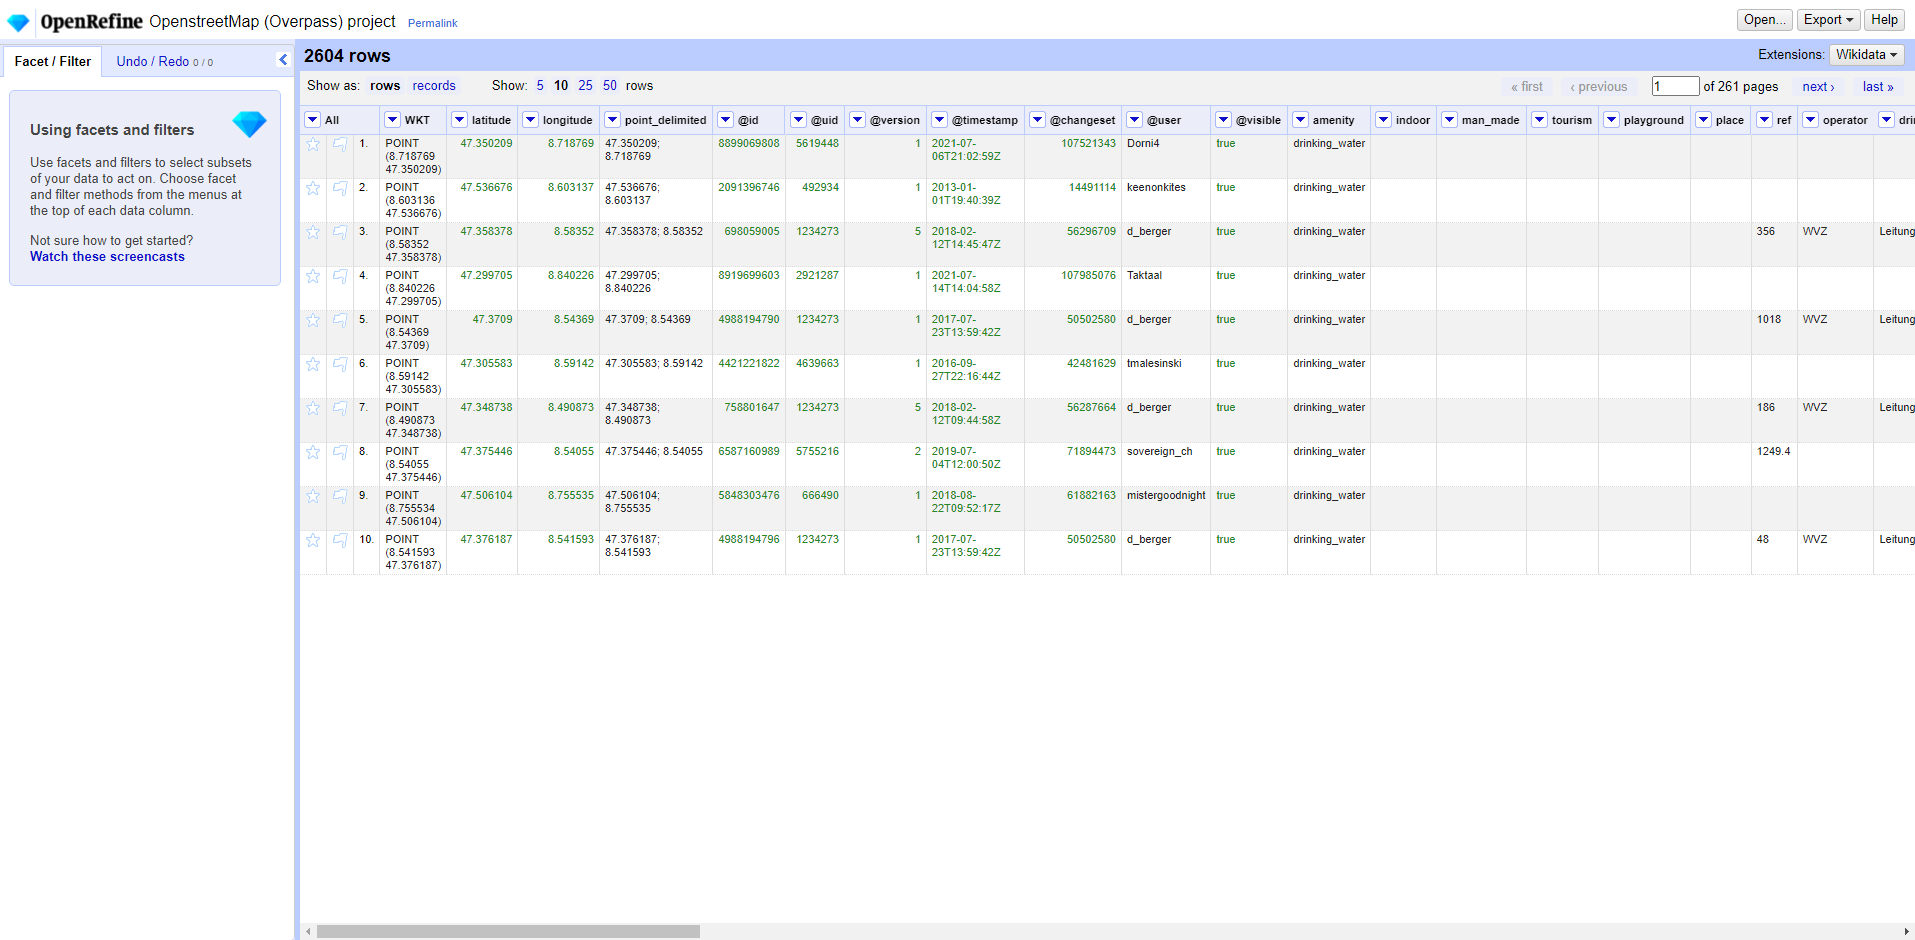
\includegraphics[width=\textwidth]{./Figures/ManagementSummary/osm_extractor_project}
    \caption{OpenRefine project created using the OSM Extractor extension, containing geometry objects for all the drinking water amenities in Zürich, Switzerland}
\end{figure}
\subsection*{The GeoJSON Export Extension}
The extension has been successfully developed using OpenRefine\textquotesingle s extension architecture and is able to successfully export
geospatial data of an OpenRefine project in the GeoJSON (.geojson) format.
\begin{figure}[H]
    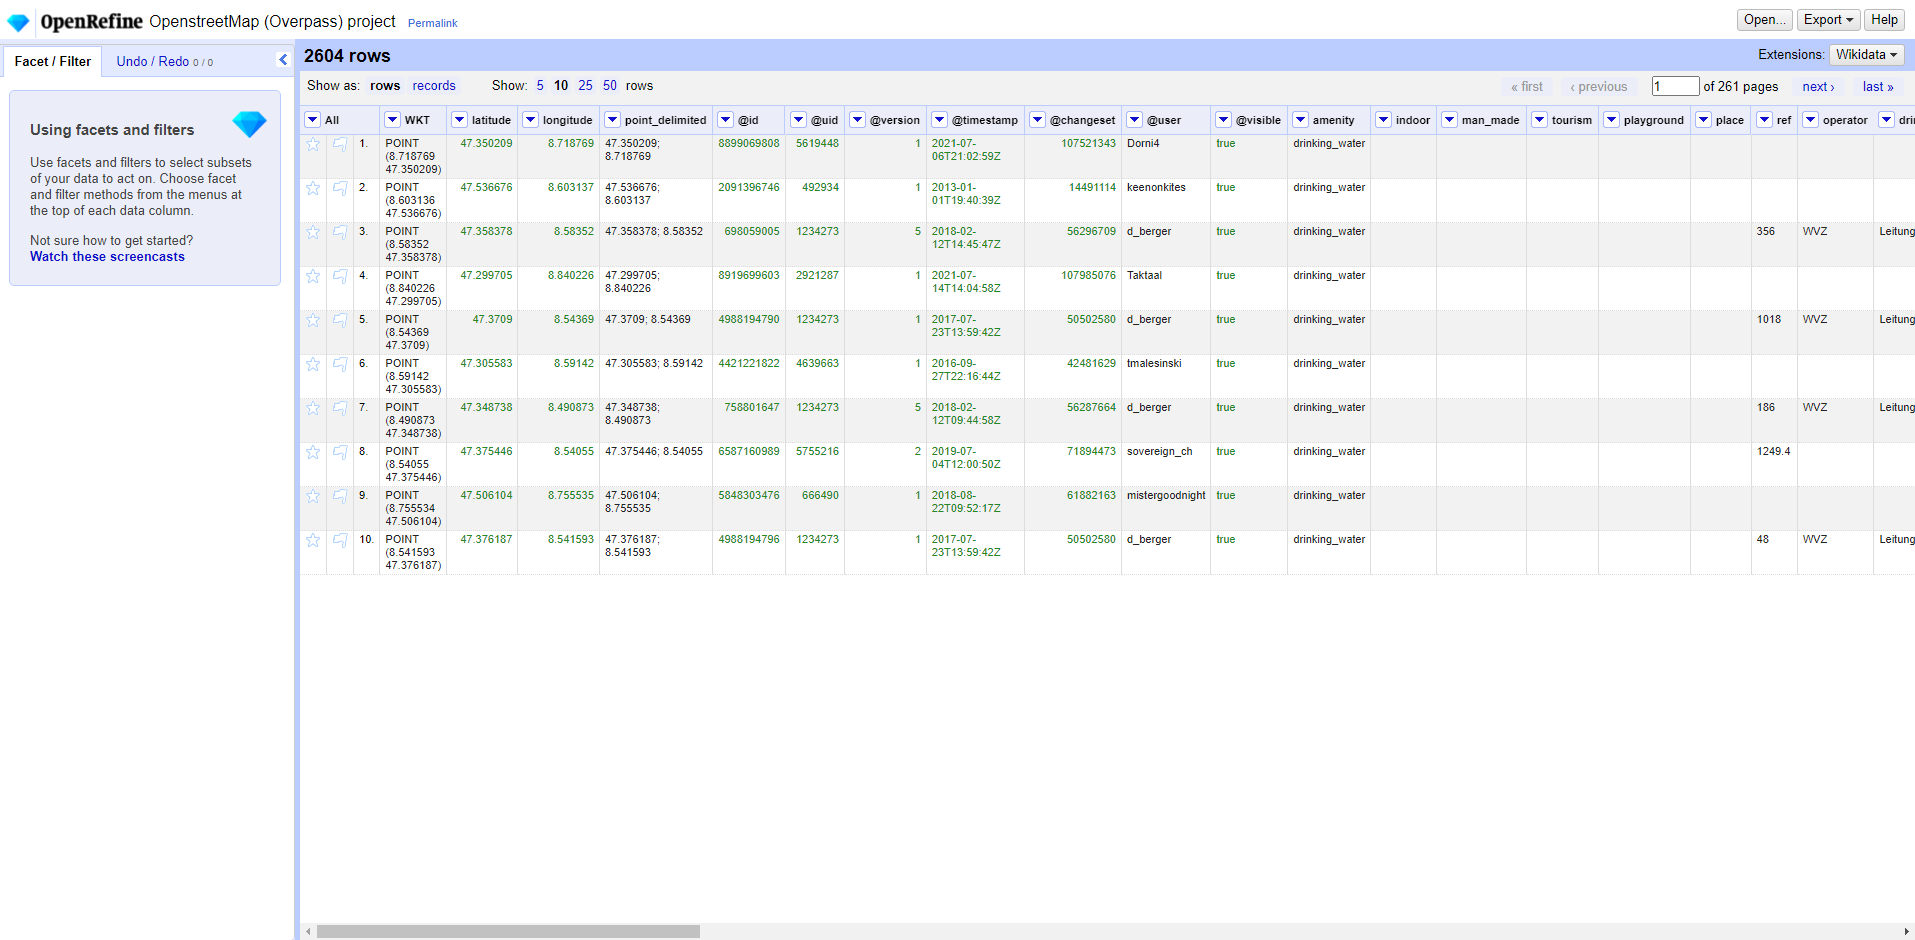
\includegraphics[width=\textwidth]{./Figures/ManagementSummary/osm_extractor_project}
    \caption{An OpenRefine project containing data for all the drinking water amenities in Zürich, Switzerland}
\end{figure}
And here is a portion of the GeoJSON exported file contents from the same project:
\begin{minted}[breaklines, tabsize=2, linenos]{json}
{
  "type" : "FeatureCollection",
  "features" : [ {
    "type" : "Feature",
    "geometry" : {
      "type" : "Point",
      "coordinates" : [ 8.718769, 47.350209 ]
    },
    "properties" : {
      "@timestamp" : "2021-07-06T21:02:59Z",
      "amenity" : "drinking_water",
      "@user" : "Dorni4",
      "@version" : "1",
      "@changeset" : "107521343",
      "@id" : "8899069808",
      "@uid" : "5619448",
      "@visible" : "true"
    }
  }, {
    "type" : "Feature",
    "geometry" : {
      "type" : "Point",
      "coordinates" : [ 8.603137, 47.536676 ]
    },
    "properties" : {
      "@timestamp" : "2013-01-01T19:40:39Z",
      "amenity" : "drinking_water",
      "@user" : "keenonkites",
      "@version" : "1",
      "@changeset" : "14491114",
      "@id" : "2091396746",
      "@uid" : "492934",
      "@visible" : "true"
    }
  }, {
    "type" : "Feature",
    "geometry" : {
      "type" : "Point",
      "coordinates" : [ 8.58352, 47.358378 ]
    },
    "properties" : {
      "@timestamp" : "2018-02-12T14:45:47Z",
      "amenity" : "drinking_water",
      "@user" : "d_berger",
      "@version" : "5",
      "@changeset" : "56296709",
      "@id" : "698059005",
      "@uid" : "1234273",
      "@visible" : "true"
    }
  } ]
}
\end{minted}
As seen in the JSON snippet above, a \mintinline{bash}{FeatureCollection} GeoJSON object is created containing all of the
\mintinline{bash}{Points} from the OpenRefine project, along with their non-spatial attributes (\textit{amenity}, \textit{@timestamp}, \textit{@id} etc.)
\pagebreak
\section*{Future Outlook}
\subsection*{The OSM Extractor Extension}
Future versions can be improved by providing an option that would continously sync that same OpenStreetMap data
with the new updates in OpenStreetMap. The user would need a \textit{Sync} button on the OpenRefine project which would
sync the current data with the latest updates/additions on the OpenStreetMap database.
\subsection*{The GeoJSON Export Extension}
Future versions of this extension could consider adding the  \mintinline{bash}{GeometryCollection} Geometry object
into the supported GeoJSON geometry types. All the other GeoJSON Geometry types are supported in the current version.